% Requires:
% \usepackage{tikz}
% \usetikzlibrary{calc}

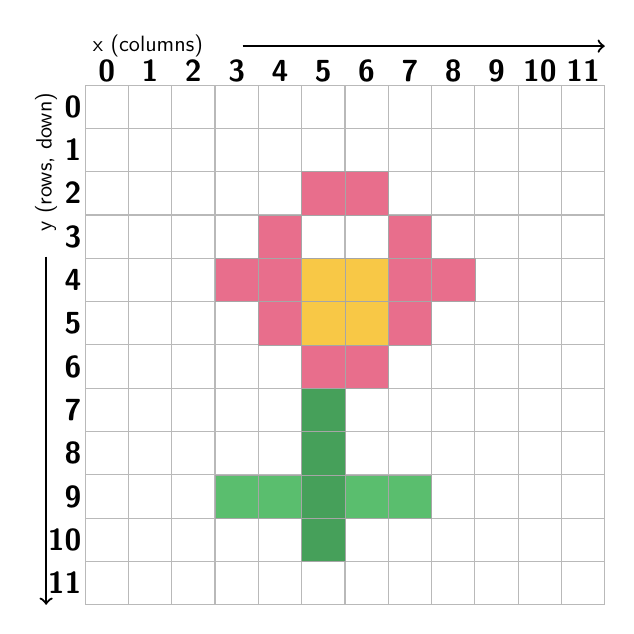
\begin{tikzpicture}[
  font=\sffamily,
  x=0.55cm, y=0.55cm, % pixel size
  line join=round
]
  % ---- grid size ----
  \def\W{12} % number of columns
  \def\H{12} % number of rows

  % ---- background ----
  \fill[white] (0,0) rectangle (\W,\H);

  % ---- draw grid ----
  \draw[step=1, gray!55] (0,0) grid (\W,\H);

  % ---- axis labels: x left->right, y top->bottom ----
  % Column indices along top: 0..W-1
  \foreach \x in {0,...,11} {
    \node[anchor=south, scale=1.1, font=\bfseries\sffamily, inner sep=1pt] at (\x+0.5, \H) {\x};
  }
  % Row indices along left, with y increasing downward:
  % Put 0 at the top row (near y=H-0.5), then 1 below it, ...
  \foreach \y in {0,...,11} {
    \node[anchor=east, scale=1.1, font=\bfseries\sffamily, inner sep=1pt] at (0, \H-\y-0.5) {\y};
  }

  % Optional axis titles
  \node[anchor=west, scale=0.8] at (0, \H+0.9) {x (columns)};
  \draw[->,line width=0.8pt] (2cm, \H+0.9) -s (\W,\H+0.9);
  \node[anchor=east, scale=0.8, rotate=90] at (-0.9, \H) {y (rows, down)}; % name this node Y
  \draw[->,line width=0.8pt] (-0.9, \H+4cm) -- (-0.9, 0); % start this at the south of Y offset by 0.5 downwards and continue it down

  % ---- helper: draw a pixel at (x,y) where y=0 is top row ----
  % We'll just place rectangles manually using the mapping:
  % pixel (x,y) -> rectangle from (x, H-y-1) to (x+1, H-y)

  % Colors
  \definecolor{petal}{RGB}{232,110,140}
  \definecolor{center}{RGB}{248,200,70}
  \definecolor{stem}{RGB}{70,160,90}
  \definecolor{leaf}{RGB}{90,190,110}

  % ---- flower pixels ----
  % petals (a chunky 5x5-ish flower head)


  % Petals (explicit, simpler)
  \foreach \x/\y in {
    5/2, 6/2,
    4/3, 7/3,
    3/4, 8/4,
    4/5, 7/5,
    5/6, 6/6,
    5/4, 6/4, 4/4, 7/4 % make it fuller
  }{
    \fill[petal] (\x, \H-\y-1) rectangle (\x+1, \H-\y);
  }

  % center
  \foreach \x/\y in {5/4,6/4,5/5,6/5} {
    \fill[center] (\x, \H-\y-1) rectangle (\x+1, \H-\y);
  }

  % stem
  \foreach \x/\y in {5/7,5/8,5/9,5/10} {
    \fill[stem] (\x, \H-\y-1) rectangle (\x+1, \H-\y);
  }

  % leaves
  \foreach \x/\y in {4/9,3/9,6/9,7/9} {
    \fill[leaf] (\x, \H-\y-1) rectangle (\x+1, \H-\y);
  }

  % ---- optional: outline the flower pixels slightly darker ----
  \foreach \x/\y in {
    5/2, 6/2,
    4/3, 7/3,
    3/4, 4/4, 5/4, 6/4, 7/4, 8/4,
    4/5, 5/5, 6/5, 7/5,
    5/6, 6/6,
    5/7,5/8,5/9,5/10,
    4/9,3/9,6/9,7/9
  }{
    \draw[black!35, line width=0.2pt] (\x, \H-\y-1) rectangle (\x+1, \H-\y);
  }

\end{tikzpicture}

